\documentclass[dvisvgm]{minimal}
\usepackage{tikz}
\usepackage{pgfplots} % for tikz plot
\usetikzlibrary{positioning,fit,calc,shadows}
\usepackage{assets/tikz/myTikz}
% \pgfrealjobname{dummy}

\begin{document}

% This file was created by matlab2tikz.
%
%The latest updates can be retrieved from
%  http://www.mathworks.com/matlabcentral/fileexchange/22022-matlab2tikz-matlab2tikz
%where you can also make suggestions and rate matlab2tikz.
%


\definecolor{mycolor1}{rgb}{0.00000,0.44700,0.74100}% Medium to dark blue (steel blue)
\definecolor{mycolor2}{rgb}{0.46600,0.67400,0.18800}% Earthy green (grass green)
% \definecolor{mycolor2}{RGB}{0, 158, 115} % Green
\colorlet{mycolor2}{mycolor2!80!black}
\definecolor{mycolor3}{rgb}{0.85000,0.32500,0.09800}% Bright orange (burnt orange)
% \definecolor{mycolor4}{HTML}{DAA520} % Goldenrod
\definecolor{mycolor4}{rgb}{0.92900,0.69400,0.12500}%
\colorlet{mycolor1}{mycolor1!80!white}%

\begin{tikzpicture}

\begin{axis}[%
  DarkMode,
  name=plot1,
  width=0.9\linewidth, % Width of the plot
  height=0.5\linewidth, % Height of the plot
  axis lines=left,
  xmin=220,
  xmax=309,
  ymin=0,
  ymax=160,
  ylabel={Direction of Arrival [$^\circ$]},
  xlabel={Time [s]},
  % title style={font=\bfseries},
  title={Tracking of elephant footsteps},
  xmajorgrids,
  ymajorgrids,
  legend style={legend cell align=left, align=center,
  at={(0.53,0.55)}, % Place legend at the top center
  anchor=south,    % Anchor the bottom of the legend box to the top center of the plot
  clip mode=individual,
  line width=1.1pt,
  axis line style={line width=1.1pt},
  }
]
\addplot [color=mycolor1, dashed, line width=1pt]
  table[row sep=crcr]{%
221.784	145\\
221.884	144.854131019432\\
221.984	144.701292337366\\
222.084	144.541612610321\\
222.184	144.375220494812\\
222.284	144.202244647357\\
222.384	144.022813724474\\
222.484	143.837056382681\\
222.584	143.645101278493\\
222.684	143.447077068428\\
222.784	143.243112409005\\
222.884	143.03333595674\\
222.984	142.817876368149\\
223.084	142.596862299752\\
223.184	142.370422408064\\
223.284	142.138685349604\\
223.384	141.901779780888\\
223.484	141.659834358434\\
223.584	141.412977738759\\
223.684	141.16133857838\\
223.784	140.905045533815\\
223.884	140.644227261581\\
223.984	140.379012418195\\
224.084	140.109529660175\\
224.184	139.835907644037\\
224.284	139.558275026299\\
224.384	139.276760463479\\
224.484	138.991492612094\\
224.584	138.70260012866\\
224.684	138.410211669695\\
224.784	138.114455891718\\
224.884	137.815461451244\\
224.984	137.513357004791\\
225.084	137.208271208876\\
225.184	136.900332720017\\
225.284	136.589670194731\\
225.384	136.276412289535\\
225.484	135.960687660947\\
225.584	135.642624965483\\
225.684	135.322352859662\\
225.784	135\\
225.884	134.675695043015\\
225.984	134.349566645223\\
226.084	134.021743463143\\
226.184	133.692354153292\\
226.284	133.361527372186\\
226.384	133.029391776343\\
226.484	132.696076022281\\
226.584	132.361708766516\\
226.684	132.026418665567\\
226.784	131.69033437595\\
226.884	131.353584554182\\
226.984	131.016297856781\\
227.084	130.678602940264\\
227.184	130.340628461149\\
227.284	130.002503075952\\
227.384	129.664355441191\\
227.484	129.326314213384\\
227.584	128.988508049047\\
227.684	128.651065604698\\
227.784	128.314115536854\\
227.884	127.977786502032\\
227.984	127.642207156751\\
228.084	127.307506157526\\
228.184	126.973812160875\\
228.284	126.641253823316\\
228.384	126.309959801366\\
228.484	125.980058751542\\
228.584	125.651679330362\\
228.684	125.324950194342\\
228.784	125\\
228.884	124.676819743173\\
228.984	124.354849776975\\
229.084	124.03339279384\\
229.184	123.711751486201\\
229.284	123.389228546493\\
229.384	123.065126667149\\
229.484	122.738748540603\\
229.584	122.409396859289\\
229.684	122.076374315641\\
229.784	121.738983602092\\
229.884	121.396527411076\\
229.984	121.048308435027\\
230.084	120.693629366378\\
230.184	120.331792897564\\
230.284	119.962101721019\\
230.384	119.583858529175\\
230.484	119.196366014467\\
230.584	118.798926869329\\
230.684	118.390843786194\\
230.784	117.971419457497\\
230.884	117.53995657567\\
230.984	117.095757833149\\
231.084	116.638125922365\\
231.184	116.166363535754\\
231.284	115.67977336575\\
231.384	115.177658104785\\
231.484	114.659320445294\\
231.584	114.12406307971\\
231.684	113.571188700467\\
231.784	113\\
231.884	112.410217625131\\
231.984	111.803234040244\\
232.084	111.180859664111\\
232.184	110.544904915505\\
232.284	109.897180213198\\
232.384	109.239495975964\\
232.484	108.573662622575\\
232.584	107.901490571804\\
232.684	107.224790242423\\
232.784	106.545372053206\\
232.884	105.865046422924\\
232.984	105.185623770351\\
233.084	104.508914514259\\
233.184	103.836729073421\\
233.284	103.17087786661\\
233.384	102.513171312598\\
233.484	101.865419830159\\
233.584	101.229433838064\\
233.684	100.607023755087\\
233.784	100\\
233.884	99.4096881542429\\
233.984	98.8354744499226\\
234.084	98.2762602818128\\
234.184	97.7309470446875\\
234.284	97.1984361333205\\
234.384	96.6776289424855\\
234.484	96.1674268669563\\
234.584	95.6667313015068\\
234.684	95.1744436409109\\
234.784	94.6894652799423\\
234.884	94.2106976133749\\
234.984	93.7370420359824\\
235.084	93.2673999425386\\
235.184	92.8006727278176\\
235.284	92.335761786593\\
235.384	91.8715685136386\\
235.484	91.4069943037284\\
235.584	90.9409405516358\\
235.684	90.4723086521352\\
235.784	90\\
235.884	89.5231547578972\\
235.984	89.0418681600658\\
236.084	88.5564742086377\\
236.184	88.0673069057451\\
236.284	87.5747002535198\\
236.384	87.0789882540941\\
236.484	86.5805049095997\\
236.584	86.0795842221686\\
236.684	85.5765601939332\\
236.784	85.0717668270253\\
236.884	84.5655381235768\\
236.984	84.0582080857198\\
237.084	83.5501107155863\\
237.184	83.0415800153084\\
237.284	82.532949987018\\
237.384	82.0245546328473\\
237.484	81.5167279549281\\
237.584	81.0098039553923\\
237.684	80.5041166363724\\
237.784	80\\
237.884	79.4977042143734\\
237.984	78.9971441114552\\
238.084	78.4981506891739\\
238.184	78.0005549454586\\
238.284	77.5041878782379\\
238.384	77.0088804854405\\
238.484	76.5144637649951\\
238.584	76.0207687148304\\
238.684	75.5276263328753\\
238.784	75.0348676170584\\
238.884	74.5423235653085\\
238.984	74.0498251755543\\
239.084	73.5572034457245\\
239.184	73.0642893737479\\
239.284	72.5709139575532\\
239.384	72.0769081950692\\
239.484	71.5821030842245\\
239.584	71.0863296229478\\
239.684	70.5894188091681\\
239.784	70.091201640814\\
239.884	69.5915091158141\\
239.984	69.0901722320973\\
240.084	68.5870219875922\\
240.184	68.0818893802276\\
240.284	67.5746054079324\\
240.384	67.065001068635\\
240.484	66.5529073602644\\
240.584	66.0381552807491\\
240.684	65.5205758280181\\
240.784	65\\
240.884	64.4763403603209\\
240.984	63.9498357353967\\
241.084	63.4208065173404\\
241.184	62.8895730982654\\
241.284	62.3564558702849\\
241.384	61.821775225512\\
241.484	61.2858515560599\\
241.584	60.7490052540417\\
241.684	60.2115567115709\\
241.784	59.6738263207605\\
241.884	59.1361344737237\\
241.984	58.5988015625737\\
242.084	58.0621479794235\\
242.184	57.5264941163867\\
242.284	56.9921603655764\\
242.384	56.4594671191056\\
242.484	55.9287347690876\\
242.584	55.4002837076355\\
242.684	54.8744343268627\\
242.784	54.3515070188823\\
242.884	53.8318221758075\\
242.984	53.3157001897514\\
243.084	52.8034614528272\\
243.184	52.2954263571484\\
243.284	51.7919152948279\\
243.384	51.293248657979\\
243.484	50.7997468387148\\
243.584	50.3117302291485\\
243.684	49.8295192213936\\
243.784	49.3534342075629\\
243.884	48.8837955797699\\
243.984	48.4209237301276\\
244.084	47.9651390507491\\
244.184	47.5167619337479\\
244.284	47.0761127712371\\
244.384	46.6435119553298\\
244.484	46.2192798781392\\
244.584	45.8037369317785\\
244.684	45.3972035083611\\
244.784	45\\
244.884	44.6123617911292\\
244.984	44.2341842354657\\
245.084	43.8652776790472\\
245.184	43.5054524679116\\
245.284	43.1545189480966\\
245.384	42.81228746564\\
245.484	42.4785683665796\\
245.584	42.1531719969529\\
245.684	41.835908702798\\
245.784	41.5265888301526\\
245.884	41.2250227250543\\
245.984	40.931020733541\\
246.084	40.6443932016504\\
246.184	40.3649504754204\\
246.284	40.0925029008886\\
246.384	39.8268608240929\\
246.484	39.567834591071\\
246.584	39.3152345478606\\
246.684	39.0688710404996\\
246.784	38.8285544150257\\
246.884	38.5940950174767\\
246.984	38.3653031938903\\
247.084	38.1419892903042\\
247.184	37.9239636527564\\
247.284	37.7110366272845\\
247.384	37.5030185599264\\
247.484	37.2997197967197\\
247.584	37.1009506837021\\
247.684	36.9065215669117\\
247.784	36.716242792386\\
247.884	36.5299247061628\\
247.984	36.34737765428\\
248.084	36.1684119827751\\
248.184	35.9928380376862\\
248.284	35.8204661650509\\
248.384	35.6511067109069\\
248.484	35.4845700212921\\
248.584	35.3206664422441\\
248.684	35.1592063198008\\
248.784	35\\
248.884	34.8429831907472\\
248.984	34.6885930474197\\
249.084	34.5373920872622\\
249.184	34.3899428275199\\
249.284	34.2468077854377\\
249.384	34.1085494782606\\
249.484	33.9757304232335\\
249.584	33.8489131376015\\
249.684	33.7286601386094\\
249.784	33.6155339435024\\
249.884	33.5100970695253\\
249.984	33.4129120339231\\
250.084	33.3245413539408\\
250.184	33.2455475468234\\
250.284	33.1764931298159\\
250.384	33.1179406201631\\
250.484	33.0704525351102\\
250.584	33.0345913919021\\
250.684	33.0109197077837\\
250.784	33\\
250.884	33\\
250.984	33.0018165055467\\
251.084	33.0031843666001\\
251.184	33.0041466426182\\
251.284	33.0047463930593\\
251.384	33.0050266773815\\
251.484	33.0050305550429\\
251.584	33.0048010855016\\
251.684	33.0043813282159\\
251.784	33.0038143426438\\
251.884	33.0031431882436\\
251.984	33.0024109244733\\
252.084	33.0016606107911\\
252.184	33.0009353066551\\
252.284	33.0002780715235\\
252.384	32.9997306776014\\
252.484	32.999308023853\\
252.584	32.9989995722607\\
252.684	32.9987937850777\\
252.784	32.9986791245568\\
252.884	32.9986440529511\\
252.984	32.9986770325134\\
253.084	32.9987665254968\\
253.184	32.9989009941543\\
253.284	32.9990689007387\\
253.384	32.9992587075032\\
253.484	32.9994588767006\\
253.584	32.9996578705839\\
253.684	32.9998441514061\\
253.784	33.0000061816022\\
253.884	33.0001351822264\\
253.984	33.0002321017951\\
254.084	33.0003000318381\\
254.184	33.0003420638854\\
254.284	33.000361289467\\
254.384	33.0003608001128\\
254.484	33.0003436873528\\
254.584	33.0003130427171\\
254.684	33.0002719577355\\
254.784	33.0002235239381\\
254.884	33.0001708328548\\
254.984	33.0001169760156\\
255.084	33.0000650449505\\
255.184	33.0000181311894\\
255.284	32.9999792095774\\
255.384	32.9999492263427\\
255.484	32.999927407575\\
255.584	32.9999129249012\\
255.684	32.9999049499486\\
255.784	32.9999026543443\\
255.884	32.9999052097154\\
255.984	32.9999117876892\\
256.084	32.9999215598926\\
256.184	32.9999336979529\\
256.284	32.9999473734972\\
256.384	32.9999617581526\\
256.484	32.9999760235463\\
256.584	32.9999893413054\\
256.684	33.0000008831616\\
256.784	33.0000100435374\\
256.884	33.0000169099436\\
256.984	33.0000217043417\\
257.084	33.000024648693\\
257.184	33.0000259649592\\
257.284	33.0000258751016\\
257.384	33.0000246010818\\
257.484	33.0000223648612\\
257.584	33.0000193884013\\
257.684	33.0000158936636\\
257.784	33.0000121026096\\
257.884	33.0000082372007\\
257.984	33.0000045193984\\
258.084	33.0000011711643\\
258.184	32.9999984040591\\
258.284	32.9999962772179\\
258.384	32.9999947340529\\
258.484	32.9999937150908\\
258.584	32.9999931608587\\
258.684	32.9999930118835\\
258.784	32.9999932086922\\
258.884	32.9999936918117\\
258.984	32.999994401769\\
259.084	32.9999952790909\\
259.184	32.9999962643046\\
259.284	32.9999972979368\\
259.384	32.9999983205146\\
259.484	32.999999272565\\
259.584	33.0000000946401\\
259.684	33.0000007451476\\
259.784	33.0000012316368\\
259.884	33.0000015700386\\
259.984	33.0000017762837\\
260.084	33.0000018663028\\
260.184	33.0000018560265\\
260.284	33.0000017613856\\
260.384	33.0000015983109\\
260.484	33.000001382733\\
260.584	33.0000011305827\\
260.684	33.0000008577906\\
260.784	33.0000005802875\\
260.884	33.0000003140042\\
260.984	33.0000000748712\\
261.084	32.9999998779069\\
261.184	32.9999997267428\\
261.284	32.9999996172764\\
261.384	32.999999545258\\
261.484	32.9999995064378\\
261.584	32.9999994965659\\
261.684	32.9999995113925\\
261.784	32.9999995466679\\
261.884	32.9999995981422\\
261.984	32.9999996615655\\
262.084	32.9999997326881\\
262.184	32.9999998072602\\
262.284	32.9999998810319\\
262.384	32.9999999497534\\
262.484	33.0000000091791\\
262.584	33.0000000564605\\
262.684	33.0000000921563\\
262.784	33.0000001173352\\
262.884	33.0000001330656\\
262.984	33.0000001404161\\
263.084	33.0000001404552\\
263.184	33.0000001342516\\
263.284	33.0000001228738\\
263.384	33.0000001073902\\
263.484	33.0000000888695\\
263.584	33.0000000683802\\
263.684	33.0000000469909\\
263.784	33.0000000257701\\
263.884	33.0000000057863\\
263.984	32.9999999880485\\
264.084	32.9999999729258\\
264.184	32.9999999603993\\
264.284	32.9999999504447\\
264.384	32.9999999430375\\
264.484	32.9999999381534\\
264.584	32.999999935768\\
264.684	32.9999999358569\\
264.784	32.9999999383958\\
264.884	32.9999999433601\\
264.984	32.9999999507257\\
265.084	32.9999999604679\\
265.184	32.9999999725626\\
265.284	32.9999999869853\\
265.384	33.0000000037101\\
265.484	33.0000000224372\\
265.584	33.0000000422732\\
265.684	33.0000000622472\\
265.784	33.000000081388\\
265.884	33.0000000987248\\
265.984	33.0000001132864\\
266.084	33.0000001241019\\
266.184	33.0000001302002\\
266.284	33.0000001306104\\
266.384	33.0000001243614\\
266.484	33.0000001104822\\
266.584	33.0000000880019\\
266.684	33.0000000559493\\
266.784	33.0000000133534\\
266.884	32.9999999595618\\
266.984	32.9999998968703\\
267.084	32.9999998291718\\
267.184	32.9999997603745\\
267.284	32.999999694387\\
267.384	32.9999996351177\\
267.484	32.9999995864751\\
267.584	32.9999995523674\\
267.684	32.9999995367033\\
267.784	32.9999995433911\\
267.884	32.9999995763393\\
267.984	32.9999996394563\\
268.084	32.9999997366505\\
268.184	32.9999998718304\\
268.284	33.0000000488545\\
268.384	33.0000002656974\\
268.484	33.0000005089884\\
268.584	33.0000007640648\\
268.684	33.000001016264\\
268.784	33.0000012509231\\
268.884	33.0000014533795\\
268.984	33.0000016089703\\
269.084	33.000001703033\\
269.184	33.0000017209047\\
269.284	33.0000016479228\\
269.384	33.0000014694245\\
269.484	33.000001170747\\
269.584	33.0000007372277\\
269.684	33.0000001542038\\
269.784	32.9999994123698\\
269.884	32.9999985455375\\
269.984	32.9999976083154\\
270.084	32.9999966554458\\
270.184	32.9999957416714\\
270.284	32.9999949217346\\
270.384	32.9999942503778\\
270.484	32.9999937823436\\
270.584	32.9999935723743\\
270.684	32.9999936752125\\
270.784	32.9999941456006\\
270.884	32.9999950382812\\
270.984	32.9999964079967\\
271.084	32.9999983094895\\
271.184	33.0000007963967\\
271.284	33.0000038330692\\
271.384	33.0000072303454\\
271.484	33.000010783918\\
271.584	33.00001428948\\
271.684	33.0000175427242\\
271.784	33.0000203393434\\
271.884	33.0000224750304\\
271.984	33.0000237454781\\
272.084	33.0000239463792\\
272.184	33.0000228734267\\
272.284	33.0000203223133\\
272.384	33.000016088732\\
272.484	33.0000099683754\\
272.584	33.0000017569365\\
272.684	32.9999913375897\\
272.784	32.9999792082533\\
272.884	32.9999661304062\\
272.984	32.9999528665347\\
273.084	32.999940179125\\
273.184	32.9999288306632\\
273.284	32.9999195836356\\
273.384	32.9999132005284\\
273.484	32.9999104438277\\
273.584	32.9999120760198\\
273.684	32.9999188595909\\
273.784	32.9999315570271\\
273.884	32.9999509308146\\
273.984	32.9999777434397\\
274.084	33.0000127344055\\
274.184	33.0000552984328\\
274.284	33.0001027652643\\
274.384	33.0001522892626\\
274.484	33.0002010247899\\
274.584	33.0002461262086\\
274.684	33.0002847478811\\
274.784	33.0003140441698\\
274.884	33.000331169437\\
274.984	33.0003332780451\\
275.084	33.0003175243565\\
275.184	33.0002810627335\\
275.284	33.0002210475386\\
275.384	33.000134633134\\
275.484	33.0000189738822\\
275.584	32.9998726411779\\
275.684	32.9997029309463\\
275.784	32.9995204568113\\
275.884	32.9993358388372\\
275.984	32.9991596970884\\
276.084	32.9990026516292\\
276.184	32.9988753225239\\
276.284	32.9987883298368\\
276.384	32.9987522936323\\
276.484	32.9987778339745\\
276.584	32.9988755709279\\
276.684	32.9990561245568\\
276.784	32.9993301149254\\
276.884	32.9997081620981\\
276.984	33.0002004303522\\
277.084	33.0007969452911\\
277.184	33.0014600786628\\
277.284	33.0021501958478\\
277.384	33.0028276622264\\
277.484	33.003452843179\\
277.584	33.003986104086\\
277.684	33.0043878103277\\
277.784	33.0046183272846\\
277.884	33.0046380203369\\
277.984	33.0044072548651\\
278.084	33.0038863962496\\
278.184	33.0030358098708\\
278.284	33.0018158611089\\
278.384	33.0001869153444\\
278.484	32.999658186268\\
278.584	33.0085238192159\\
278.684	33.029284137815\\
278.784	33.0615428565623\\
278.884	33.1049015055281\\
278.984	33.1589616147831\\
279.084	33.2233247143978\\
279.184	33.2975923344427\\
279.284	33.3813660049883\\
279.384	33.4742472561052\\
279.484	33.5758376178638\\
279.584	33.6857386203347\\
279.684	33.8035517935884\\
279.784	33.9288786676955\\
279.884	34.0613207727264\\
279.984	34.2004796387518\\
280.084	34.3459567958421\\
280.184	34.4973537740677\\
280.284	34.6542721034994\\
280.384	34.8163133142075\\
280.484	34.9830789362627\\
280.584	35.1541965836967\\
280.684	35.3294349529274\\
280.784	35.508610221054\\
280.884	35.691538600956\\
280.984	35.8780363055132\\
281.084	36.0679195476051\\
281.184	36.2610045401112\\
281.284	36.4571074959114\\
281.384	36.6560446278851\\
281.484	36.8576321489121\\
281.584	37.0616862718718\\
281.684	37.2680232096439\\
281.784	37.4764591751082\\
281.884	37.686810381144\\
281.984	37.8988930406312\\
282.084	38.1125233664493\\
282.184	38.3275175714778\\
282.284	38.5436918685966\\
282.384	38.760862470685\\
282.484	38.978845590623\\
282.584	39.1974574412899\\
282.684	39.4165142355653\\
282.784	39.635832186329\\
282.884	39.8552275064605\\
282.984	40.0745164088396\\
283.084	40.2935151063458\\
283.184	40.5120398118585\\
283.284	40.7299067382577\\
283.384	40.9469320984227\\
283.484	41.1629321052334\\
283.584	41.3777229715693\\
283.684	41.5911209103099\\
283.784	41.8029421343349\\
283.884	42.013002856524\\
283.984	42.2211192897567\\
284.084	42.4271076469128\\
284.184	42.6307841408716\\
284.284	42.8319649845131\\
284.384	43.0304663907166\\
284.484	43.2261045723619\\
284.584	43.4186957423286\\
284.684	43.6080561134962\\
284.784	43.7940018987444\\
284.884	43.9763493109528\\
284.984	44.1549145630012\\
285.084	44.329513867769\\
285.184	44.4999634381357\\
285.284	44.6660794869813\\
285.384	44.8276782271851\\
285.484	44.9845758716269\\
285.584	45.1366560916966\\
285.684	45.2841674269683\\
285.784	45.4274812118632\\
285.884	45.5669688733377\\
285.984	45.7030018383485\\
286.084	45.8359515338522\\
286.184	45.9661893868052\\
286.284	46.0940868241644\\
286.384	46.2200152728862\\
286.484	46.3443461599273\\
286.584	46.4674509122443\\
286.684	46.5897009567936\\
286.784	46.7114677205322\\
286.884	46.8331226304163\\
286.984	46.9550371134028\\
287.084	47.0775825964481\\
287.184	47.2011305065088\\
287.284	47.3260522705417\\
287.384	47.4527193155032\\
287.484	47.5815030683501\\
287.584	47.7127749560388\\
287.684	47.846906405526\\
287.784	47.9842688437683\\
287.884	48.1252336977222\\
287.984	48.2701723943445\\
288.084	48.4194563605917\\
288.184	48.5734570234203\\
288.284	48.7325458097871\\
288.384	48.8970941466484\\
288.484	49.0674734609612\\
288.584	49.2440551796819\\
288.684	49.4272107297669\\
288.784	49.6173115381732\\
288.884	49.8147290318571\\
288.984	50.0198346377753\\
289.084	50.2329997828845\\
289.184	50.4545958941411\\
289.284	50.6849943985019\\
289.384	50.9245667229233\\
289.484	51.1736842943622\\
289.584	51.4327185397749\\
289.684	51.7020408861181\\
289.784	51.9820227603485\\
289.884	52.2730355894224\\
289.984	52.5754508002969\\
290.084	52.8896398199282\\
290.184	53.2159740752729\\
290.284	53.554824993288\\
290.384	53.9065640009295\\
290.484	54.2715625251546\\
290.584	54.6501919929196\\
290.684	55.0428238311809\\
290.784	55.4498294668956\\
290.884	55.8715803270198\\
290.984	56.3084478385106\\
291.084	56.7608034283243\\
291.184	57.2290185234173\\
291.284	57.7134645507467\\
291.384	58.2145129372686\\
291.484	58.73253510994\\
291.584	59.2679024957175\\
291.684	59.8209865215572\\
291.784	60.3921586144163\\
291.884	60.9817902012509\\
291.984	61.5902527090181\\
292.084	62.2179175646744\\
292.184	62.8651561951758\\
292.284	63.5323400274797\\
292.384	64.219840488542\\
292.484	64.9280290053201\\
292.584	65.6569006727178\\
292.684	66.4044150886807\\
292.784	67.1678468132497\\
292.884	67.9444698902335\\
292.984	68.7315583634424\\
293.084	69.5263862766856\\
293.184	70.326227673772\\
293.284	71.1283565985121\\
293.384	71.9300470947146\\
293.484	72.7285732061897\\
293.584	73.5212089767466\\
293.684	74.3052284501944\\
293.784	75.0779056703434\\
293.884	75.8365146810023\\
293.984	76.5783295259814\\
294.084	77.3006242490898\\
294.184	78.0006728941366\\
294.284	78.6757495049322\\
294.384	79.3231281252853\\
294.484	79.9400827990061\\
294.584	80.5244108775401\\
294.684	81.0767401677648\\
294.784	81.5986510543824\\
294.884	82.0917246399369\\
294.984	82.5575420269733\\
295.084	82.9976843180361\\
295.184	83.4137326156694\\
295.284	83.8072680224186\\
295.384	84.1798716408276\\
295.484	84.5331245734414\\
295.584	84.8686079228046\\
295.684	85.1879027914613\\
295.784	85.4925902819567\\
295.884	85.784251496835\\
295.984	86.064467538641\\
296.084	86.3348195099192\\
296.184	86.5968885132141\\
296.284	86.8522556510705\\
296.384	87.1025020260327\\
296.484	87.3492087406457\\
296.584	87.5939568974537\\
296.684	87.8383275990014\\
296.784	88.0839019478336\\
296.884	88.3322610464945\\
296.984	88.584985997529\\
297.084	88.8436579034817\\
297.184	89.1098578668968\\
297.284	89.3851669903194\\
297.384	89.6711663762938\\
297.484	89.9694371273647\\
297.584	90.2814658690702\\
297.684	90.6082282216861\\
297.784	90.9505278288252\\
297.884	91.3091682045017\\
297.984	91.6849528627305\\
298.084	92.0786853175259\\
298.184	92.4911690829022\\
298.284	92.9232076728744\\
298.384	93.3756046014565\\
298.484	93.8491633826636\\
298.584	94.3446875305098\\
298.684	94.8629805590095\\
298.784	95.4048459821776\\
298.884	95.9710873140282\\
298.984	96.5625080685763\\
299.084	97.1799117598362\\
299.184	97.824101901822\\
299.284	98.495882008549\\
299.384	99.1960555940309\\
299.484	99.925426172283\\
299.584	100.684355604735\\
299.684	101.470816951523\\
299.784	102.2819793318\\
299.884	103.115011258882\\
299.984	103.967081246085\\
300.084	104.835357806727\\
300.184	105.717009454124\\
300.284	106.609204701594\\
300.384	107.509112062452\\
300.484	108.413900050017\\
300.584	109.320737177605\\
300.684	110.226791958532\\
300.784	111.129232906116\\
300.884	112.025228533673\\
300.984	112.911947354522\\
301.084	113.786944106061\\
301.184	114.649862526467\\
301.284	115.501049398302\\
301.384	116.340852033931\\
301.484	117.169617745716\\
301.584	117.987693846021\\
301.684	118.79542764721\\
301.784	119.593166461646\\
301.884	120.381257601693\\
301.984	121.160048379714\\
302.084	121.929886108072\\
302.184	122.691118099131\\
302.284	123.444091665256\\
302.384	124.189154118807\\
302.484	124.926652772151\\
302.584	125.656851971021\\
302.684	126.37956731298\\
302.784	127.094463371287\\
302.884	127.801204605395\\
302.984	128.499455474755\\
303.084	129.188880438818\\
303.184	129.869143957036\\
303.284	130.539910488859\\
303.384	131.20084449374\\
303.484	131.851610431129\\
303.584	132.491872760478\\
303.684	133.121295941239\\
303.784	133.739544432863\\
303.884	134.3462826948\\
303.984	134.941175186504\\
304.084	135.523886367424\\
304.184	136.094080697012\\
304.284	136.651422634721\\
304.384	137.19557664\\
304.484	137.726207172302\\
304.584	138.242978691078\\
304.684	138.745555655778\\
304.784	139.233602525856\\
304.884	139.706783760761\\
304.984	140.164763819946\\
305.084	140.607207162861\\
305.184	141.033778248958\\
305.284	141.444141537689\\
305.384	141.837961488505\\
305.484	142.214902560857\\
305.584	142.574629214197\\
305.684	142.916805907976\\
305.784	143.241097101645\\
305.884	143.547167254656\\
305.984	143.83468082646\\
306.084	144.103302276508\\
306.184	144.352696064252\\
306.284	144.582526649144\\
306.384	144.792458490634\\
306.484	144.982156048174\\
};
\addlegendentry{Estimate from video}
\addplot [color=mycolor4, line width=1pt, forget plot]
  table[row sep=crcr]{%
-225.086471	123.949747202006\\
-325.086471	123.949747202006\\};

\addplot [color=mycolor2, line width=0.8pt, only marks, mark size=2.0pt, mark=asterisk, mark options={solid, mycolor2}, forget plot]
 plot [error bars/.cd, y dir=both, y explicit, error bar style={line width=0.8pt}, error mark options={line width=0.8pt, mark size=1.5pt, rotate=90}]
 table[row sep=crcr, y error plus index=2, y error minus index=2]{%
225.086471	123.949747202006	8.25283632357407	8.25283632357407\\
};
\addplot [color=mycolor2, line width=0.8pt, only marks, mark size=2.0pt, mark=asterisk, mark options={solid, mycolor2}, forget plot]
 plot [error bars/.cd, y dir=both, y explicit, error bar style={line width=0.8pt}, error mark options={line width=0.8pt, mark size=1.5pt, rotate=90}]
 table[row sep=crcr, y error plus index=2, y error minus index=3]{%
225.456671	121.696094298107	8.57107910926115	8.57107910926115\\
};
\addplot [color=mycolor2, line width=0.8pt, only marks, mark size=2.0pt, mark=asterisk, mark options={solid, mycolor2}, forget plot]
 plot [error bars/.cd, y dir=both, y explicit, error bar style={line width=0.8pt}, error mark options={line width=0.8pt, mark size=1.5pt, rotate=90}]
 table[row sep=crcr, y error plus index=2, y error minus index=3]{%
225.826886	136.278786765633	11.3809047793591	11.3809047793591\\
};
\addplot [color=mycolor2, line width=0.8pt, only marks, mark size=2.0pt, mark=asterisk, mark options={solid, mycolor2}, forget plot]
 plot [error bars/.cd, y dir=both, y explicit, error bar style={line width=0.8pt}, error mark options={line width=0.8pt, mark size=1.5pt, rotate=90}]
 table[row sep=crcr, y error plus index=2, y error minus index=3]{%
226.567261	118.611260054172	6.9860572886095	6.9860572886095\\
};
\addplot [color=mycolor2, line width=0.8pt, only marks, mark size=2.0pt, mark=asterisk, mark options={solid, mycolor2}, forget plot]
 plot [error bars/.cd, y dir=both, y explicit, error bar style={line width=0.8pt}, error mark options={line width=0.8pt, mark size=1.5pt, rotate=90}]
 table[row sep=crcr, y error plus index=2, y error minus index=3]{%
226.937443	116.629268421045	7.49030883183527	7.49030883183527\\
};
\addplot [color=mycolor2, line width=0.8pt, only marks, mark size=2.0pt, mark=asterisk, mark options={solid, mycolor2}, forget plot]
 plot [error bars/.cd, y dir=both, y explicit, error bar style={line width=0.8pt}, error mark options={line width=0.8pt, mark size=1.5pt, rotate=90}]
 table[row sep=crcr, y error plus index=2, y error minus index=3]{%
228.048081	107.519388820662	8.20578130268546	8.20578130268546\\
};
\addplot [color=mycolor2, line width=0.8pt, only marks, mark size=2.0pt, mark=asterisk, mark options={solid, mycolor2}, forget plot]
 plot [error bars/.cd, y dir=both, y explicit, error bar style={line width=0.8pt}, error mark options={line width=0.8pt, mark size=1.5pt, rotate=90}]
 table[row sep=crcr, y error plus index=2, y error minus index=3]{%
229.158658	106.473586257332	7.53942679009292	7.53942679009292\\
};
\addplot [color=mycolor2, line width=0.8pt, only marks, mark size=2.0pt, mark=asterisk, mark options={solid, mycolor2}, forget plot]
 plot [error bars/.cd, y dir=both, y explicit, error bar style={line width=0.8pt}, error mark options={line width=0.8pt, mark size=1.5pt, rotate=90}]
 table[row sep=crcr, y error plus index=2, y error minus index=3]{%
230.269286	98.0014537534138	8.5190544226373	8.5190544226373\\
};
\addplot [color=mycolor2, line width=0.8pt, only marks, mark size=2.0pt, mark=asterisk, mark options={solid, mycolor2}, forget plot]
 plot [error bars/.cd, y dir=both, y explicit, error bar style={line width=0.8pt}, error mark options={line width=0.8pt, mark size=1.5pt, rotate=90}]
 table[row sep=crcr, y error plus index=2, y error minus index=3]{%
230.639459	76.3039383492075	9.89248330738064	9.89248330738064\\
};
\addplot [color=mycolor2, line width=0.8pt, only marks, mark size=2.0pt, mark=asterisk, mark options={solid, mycolor2}, forget plot]
 plot [error bars/.cd, y dir=both, y explicit, error bar style={line width=0.8pt}, error mark options={line width=0.8pt, mark size=1.5pt, rotate=90}]
 table[row sep=crcr, y error plus index=2, y error minus index=3]{%
231.379889	98.4041584720541	7.81228747535467	7.81228747535467\\
};
\addplot [color=mycolor2, line width=0.8pt, only marks, mark size=2.0pt, mark=asterisk, mark options={solid, mycolor2}, forget plot]
 plot [error bars/.cd, y dir=both, y explicit, error bar style={line width=0.8pt}, error mark options={line width=0.8pt, mark size=1.5pt, rotate=90}]
 table[row sep=crcr, y error plus index=2, y error minus index=3]{%
232.120264	93.2668947169502	5.69870833331153	5.69870833331153\\
};
\addplot [color=mycolor2, line width=0.8pt, only marks, mark size=2.0pt, mark=asterisk, mark options={solid, mycolor2}, forget plot]
 plot [error bars/.cd, y dir=both, y explicit, error bar style={line width=0.8pt}, error mark options={line width=0.8pt, mark size=1.5pt, rotate=90}]
 table[row sep=crcr, y error plus index=2, y error minus index=3]{%
232.490477	89.4437705920569	7.70103441185774	7.70103441185774\\
};
\addplot [color=mycolor2, line width=0.8pt, only marks, mark size=2.0pt, mark=asterisk, mark options={solid, mycolor2}, forget plot]
 plot [error bars/.cd, y dir=both, y explicit, error bar style={line width=0.8pt}, error mark options={line width=0.8pt, mark size=1.5pt, rotate=90}]
 table[row sep=crcr, y error plus index=2, y error minus index=3]{%
233.601066	77.2694747409574	8.31978248810758	8.31978248810758\\
};
\addplot [color=mycolor2, line width=0.8pt, only marks, mark size=2.0pt, mark=asterisk, mark options={solid, mycolor2}, forget plot]
 plot [error bars/.cd, y dir=both, y explicit, error bar style={line width=0.8pt}, error mark options={line width=0.8pt, mark size=1.5pt, rotate=90}]
 table[row sep=crcr, y error plus index=2, y error minus index=3]{%
233.971272	93.0824550018847	10.8023258242588	10.8023258242588\\
};
\addplot [color=mycolor2, line width=0.8pt, only marks, mark size=2.0pt, mark=asterisk, mark options={solid, mycolor2}, forget plot]
 plot [error bars/.cd, y dir=both, y explicit, error bar style={line width=0.8pt}, error mark options={line width=0.8pt, mark size=1.5pt, rotate=90}]
 table[row sep=crcr, y error plus index=2, y error minus index=3]{%
234.341478	96.8720951670535	7.22878359281369	7.22878359281369\\
};
\addplot [color=mycolor2, line width=0.8pt, only marks, mark size=2.0pt, mark=asterisk, mark options={solid, mycolor2}, forget plot]
 plot [error bars/.cd, y dir=both, y explicit, error bar style={line width=0.8pt}, error mark options={line width=0.8pt, mark size=1.5pt, rotate=90}]
 table[row sep=crcr, y error plus index=2, y error minus index=3]{%
234.71168	97.0576621248699	7.03393570487807	7.03393570487807\\
};
\addplot [color=mycolor2, line width=0.8pt, only marks, mark size=2.0pt, mark=asterisk, mark options={solid, mycolor2}, forget plot]
 plot [error bars/.cd, y dir=both, y explicit, error bar style={line width=0.8pt}, error mark options={line width=0.8pt, mark size=1.5pt, rotate=90}]
 table[row sep=crcr, y error plus index=2, y error minus index=3]{%
235.822267	96.0328046285857	5.82281892015058	5.82281892015058\\
};
\addplot [color=mycolor2, line width=0.8pt, only marks, mark size=2.0pt, mark=asterisk, mark options={solid, mycolor2}, forget plot]
 plot [error bars/.cd, y dir=both, y explicit, error bar style={line width=0.8pt}, error mark options={line width=0.8pt, mark size=1.5pt, rotate=90}]
 table[row sep=crcr, y error plus index=2, y error minus index=3]{%
236.192454	73.6050155479212	8.59376562901481	8.59376562901481\\
};
\addplot [color=mycolor2, line width=0.8pt, only marks, mark size=2.0pt, mark=asterisk, mark options={solid, mycolor2}, forget plot]
 plot [error bars/.cd, y dir=both, y explicit, error bar style={line width=0.8pt}, error mark options={line width=0.8pt, mark size=1.5pt, rotate=90}]
 table[row sep=crcr, y error plus index=2, y error minus index=3]{%
236.562643	77.0602790866851	7.40022456929646	7.40022456929646\\
};
\addplot [color=mycolor2, line width=0.8pt, only marks, mark size=2.0pt, mark=asterisk, mark options={solid, mycolor2}, forget plot]
 plot [error bars/.cd, y dir=both, y explicit, error bar style={line width=0.8pt}, error mark options={line width=0.8pt, mark size=1.5pt, rotate=90}]
 table[row sep=crcr, y error plus index=2, y error minus index=3]{%
236.932854	77.1223439383505	7.50458620643867	7.50458620643867\\
};
\addplot [color=mycolor2, line width=0.8pt, only marks, mark size=2.0pt, mark=asterisk, mark options={solid, mycolor2}, forget plot]
 plot [error bars/.cd, y dir=both, y explicit, error bar style={line width=0.8pt}, error mark options={line width=0.8pt, mark size=1.5pt, rotate=90}]
 table[row sep=crcr, y error plus index=2, y error minus index=3]{%
238.413609	67.4713743981126	8.3133636455549	8.3133636455549\\
};
\addplot [color=mycolor2, line width=0.8pt, only marks, mark size=2.0pt, mark=asterisk, mark options={solid, mycolor2}, forget plot]
 plot [error bars/.cd, y dir=both, y explicit, error bar style={line width=0.8pt}, error mark options={line width=0.8pt, mark size=1.5pt, rotate=90}]
 table[row sep=crcr, y error plus index=2, y error minus index=3]{%
239.894356	66.3868000169647	5.56404494250513	5.56404494250513\\
};
\addplot [color=mycolor2, line width=0.8pt, only marks, mark size=2.0pt, mark=asterisk, mark options={solid, mycolor2}, forget plot]
 plot [error bars/.cd, y dir=both, y explicit, error bar style={line width=0.8pt}, error mark options={line width=0.8pt, mark size=1.5pt, rotate=90}]
 table[row sep=crcr, y error plus index=2, y error minus index=3]{%
241.005021	63.537985272046	6.26038499408084	6.26038499408084\\
};
\addplot [color=mycolor2, line width=0.8pt, only marks, mark size=2.0pt, mark=asterisk, mark options={solid, mycolor2}, forget plot]
 plot [error bars/.cd, y dir=both, y explicit, error bar style={line width=0.8pt}, error mark options={line width=0.8pt, mark size=1.5pt, rotate=90}]
 table[row sep=crcr, y error plus index=2, y error minus index=3]{%
242.115616	53.4436630168286	7.4360479213997	7.4360479213997\\
};
\addplot [color=mycolor2, line width=0.8pt, only marks, mark size=2.0pt, mark=asterisk, mark options={solid, mycolor2}, forget plot]
 plot [error bars/.cd, y dir=both, y explicit, error bar style={line width=0.8pt}, error mark options={line width=0.8pt, mark size=1.5pt, rotate=90}]
 table[row sep=crcr, y error plus index=2, y error minus index=3]{%
242.855976	60.0206890870882	7.06464908349762	7.06464908349762\\
};
\addplot [color=mycolor2, line width=0.8pt, only marks, mark size=2.0pt, mark=asterisk, mark options={solid, mycolor2}, forget plot]
 plot [error bars/.cd, y dir=both, y explicit, error bar style={line width=0.8pt}, error mark options={line width=0.8pt, mark size=1.5pt, rotate=90}]
 table[row sep=crcr, y error plus index=2, y error minus index=3]{%
244.706984	50.3756542250368	7.60062365663154	7.60062365663154\\
};
\addplot [color=mycolor2, line width=0.8pt, only marks, mark size=2.0pt, mark=asterisk, mark options={solid, mycolor2}, forget plot]
 plot [error bars/.cd, y dir=both, y explicit, error bar style={line width=0.8pt}, error mark options={line width=0.8pt, mark size=1.5pt, rotate=90}]
 table[row sep=crcr, y error plus index=2, y error minus index=3]{%
246.558009	48.8059182651727	7.70337524781191	7.70337524781191\\
};
\addplot [color=mycolor2, line width=0.8pt, only marks, mark size=2.0pt, mark=asterisk, mark options={solid, mycolor2}, forget plot]
 plot [error bars/.cd, y dir=both, y explicit, error bar style={line width=0.8pt}, error mark options={line width=0.8pt, mark size=1.5pt, rotate=90}]
 table[row sep=crcr, y error plus index=2, y error minus index=3]{%
247.298356	44.7952278309065	6.31263180613382	6.31263180613382\\
};
\addplot [color=mycolor2, line width=0.8pt, only marks, mark size=2.0pt, mark=asterisk, mark options={solid, mycolor2}, forget plot]
 plot [error bars/.cd, y dir=both, y explicit, error bar style={line width=0.8pt}, error mark options={line width=0.8pt, mark size=1.5pt, rotate=90}]
 table[row sep=crcr, y error plus index=2, y error minus index=3]{%
248.038817	35.5888865461995	5.18419507499779	5.18419507499779\\
};
\addplot [color=mycolor2, line width=0.8pt, only marks, mark size=2.0pt, mark=asterisk, mark options={solid, mycolor2}, forget plot]
 plot [error bars/.cd, y dir=both, y explicit, error bar style={line width=0.8pt}, error mark options={line width=0.8pt, mark size=1.5pt, rotate=90}]
 table[row sep=crcr, y error plus index=2, y error minus index=3]{%
249.14945	41.3497646816685	7.36293151995796	7.36293151995796\\
};
\addplot [color=mycolor2, line width=0.8pt, only marks, mark size=2.0pt, mark=asterisk, mark options={solid, mycolor2}, forget plot]
 plot [error bars/.cd, y dir=both, y explicit, error bar style={line width=0.8pt}, error mark options={line width=0.8pt, mark size=1.5pt, rotate=90}]
 table[row sep=crcr, y error plus index=2, y error minus index=3]{%
249.519658	42.081569260267	7.7888810201657	7.7888810201657\\
};
\addplot [color=mycolor2, line width=0.8pt, only marks, mark size=2.0pt, mark=asterisk, mark options={solid, mycolor2}, forget plot]
 plot [error bars/.cd, y dir=both, y explicit, error bar style={line width=0.8pt}, error mark options={line width=0.8pt, mark size=1.5pt, rotate=90}]
 table[row sep=crcr, y error plus index=2, y error minus index=3]{%
250.260065	42.4837758501445	6.92760217505292	6.92760217505292\\
};
\addplot [color=mycolor2, line width=0.8pt, only marks, mark size=2.0pt, mark=asterisk, mark options={solid, mycolor2}, forget plot]
 plot [error bars/.cd, y dir=both, y explicit, error bar style={line width=0.8pt}, error mark options={line width=0.8pt, mark size=1.5pt, rotate=90}]
 table[row sep=crcr, y error plus index=2, y error minus index=3]{%
282.251845	51.0803237115438	8.18162887621959	8.18162887621959\\
};
\addplot [color=mycolor2, line width=0.8pt, only marks, mark size=2.0pt, mark=asterisk, mark options={solid, mycolor2}, forget plot]
 plot [error bars/.cd, y dir=both, y explicit, error bar style={line width=0.8pt}, error mark options={line width=0.8pt, mark size=1.5pt, rotate=90}]
 table[row sep=crcr, y error plus index=2, y error minus index=3]{%
283.732696	38.2391944412579	5.64317542684294	5.64317542684294\\
};
\addplot [color=mycolor2, line width=0.8pt, only marks, mark size=2.0pt, mark=asterisk, mark options={solid, mycolor2}, forget plot]
 plot [error bars/.cd, y dir=both, y explicit, error bar style={line width=0.8pt}, error mark options={line width=0.8pt, mark size=1.5pt, rotate=90}]
 table[row sep=crcr, y error plus index=2, y error minus index=3]{%
284.473142	53.5425243421041	8.98685862276411	8.98685862276411\\
};
\addplot [color=mycolor2, line width=0.8pt, only marks, mark size=2.0pt, mark=asterisk, mark options={solid, mycolor2}, forget plot]
 plot [error bars/.cd, y dir=both, y explicit, error bar style={line width=0.8pt}, error mark options={line width=0.8pt, mark size=1.5pt, rotate=90}]
 table[row sep=crcr, y error plus index=2, y error minus index=3]{%
284.843357	54.0136265946406	8.66180208318558	8.66180208318558\\
};
\addplot [color=mycolor2, line width=0.8pt, only marks, mark size=2.0pt, mark=asterisk, mark options={solid, mycolor2}, forget plot]
 plot [error bars/.cd, y dir=both, y explicit, error bar style={line width=0.8pt}, error mark options={line width=0.8pt, mark size=1.5pt, rotate=90}]
 table[row sep=crcr, y error plus index=2, y error minus index=3]{%
285.953997	43.0085006774619	6.79844114923196	6.79844114923196\\
};
\addplot [color=mycolor2, line width=0.8pt, only marks, mark size=2.0pt, mark=asterisk, mark options={solid, mycolor2}, forget plot]
 plot [error bars/.cd, y dir=both, y explicit, error bar style={line width=0.8pt}, error mark options={line width=0.8pt, mark size=1.5pt, rotate=90}]
 table[row sep=crcr, y error plus index=2, y error minus index=3]{%
287.06463	56.0831406788215	7.95425728017621	7.95425728017621\\
};
\addplot [color=mycolor2, line width=0.8pt, only marks, mark size=2.0pt, mark=asterisk, mark options={solid, mycolor2}, forget plot]
 plot [error bars/.cd, y dir=both, y explicit, error bar style={line width=0.8pt}, error mark options={line width=0.8pt, mark size=1.5pt, rotate=90}]
 table[row sep=crcr, y error plus index=2, y error minus index=3]{%
288.175265	48.7856322459265	8.11926071648608	8.11926071648608\\
};
\addplot [color=mycolor2, line width=0.8pt, only marks, mark size=2.0pt, mark=asterisk, mark options={solid, mycolor2}, forget plot]
 plot [error bars/.cd, y dir=both, y explicit, error bar style={line width=0.8pt}, error mark options={line width=0.8pt, mark size=1.5pt, rotate=90}]
 table[row sep=crcr, y error plus index=2, y error minus index=3]{%
288.915696	58.9142622130897	7.68801298208124	7.68801298208124\\
};
\addplot [color=mycolor2, line width=0.8pt, only marks, mark size=2.0pt, mark=asterisk, mark options={solid, mycolor2}, forget plot]
 plot [error bars/.cd, y dir=both, y explicit, error bar style={line width=0.8pt}, error mark options={line width=0.8pt, mark size=1.5pt, rotate=90}]
 table[row sep=crcr, y error plus index=2, y error minus index=3]{%
289.285911	61.0164650713634	7.99449249729455	7.99449249729455\\
};
\addplot [color=mycolor2, line width=0.8pt, only marks, mark size=2.0pt, mark=asterisk, mark options={solid, mycolor2}, forget plot]
 plot [error bars/.cd, y dir=both, y explicit, error bar style={line width=0.8pt}, error mark options={line width=0.8pt, mark size=1.5pt, rotate=90}]
 table[row sep=crcr, y error plus index=2, y error minus index=3]{%
290.026335	55.5645641499713	6.55791083200717	6.55791083200717\\
};
\addplot [color=mycolor2, line width=0.8pt, only marks, mark size=2.0pt, mark=asterisk, mark options={solid, mycolor2}, forget plot]
 plot [error bars/.cd, y dir=both, y explicit, error bar style={line width=0.8pt}, error mark options={line width=0.8pt, mark size=1.5pt, rotate=90}]
 table[row sep=crcr, y error plus index=2, y error minus index=3]{%
290.396548	55.1721816744773	6.87432439139824	6.87432439139824\\
};
\addplot [color=mycolor2, line width=0.8pt, only marks, mark size=2.0pt, mark=asterisk, mark options={solid, mycolor2}, forget plot]
 plot [error bars/.cd, y dir=both, y explicit, error bar style={line width=0.8pt}, error mark options={line width=0.8pt, mark size=1.5pt, rotate=90}]
 table[row sep=crcr, y error plus index=2, y error minus index=3]{%
291.136954	62.7988649795801	7.23151538583967	7.23151538583967\\
};
\addplot [color=mycolor2, line width=0.8pt, only marks, mark size=2.0pt, mark=asterisk, mark options={solid, mycolor2}, forget plot]
 plot [error bars/.cd, y dir=both, y explicit, error bar style={line width=0.8pt}, error mark options={line width=0.8pt, mark size=1.5pt, rotate=90}]
 table[row sep=crcr, y error plus index=2, y error minus index=3]{%
291.507157	59.3143860721303	7.9944158931253	7.9944158931253\\
};
\addplot [color=mycolor2, line width=0.8pt, only marks, mark size=2.0pt, mark=asterisk, mark options={solid, mycolor2}, forget plot]
 plot [error bars/.cd, y dir=both, y explicit, error bar style={line width=0.8pt}, error mark options={line width=0.8pt, mark size=1.5pt, rotate=90}]
 table[row sep=crcr, y error plus index=2, y error minus index=3]{%
292.247559	63.1596864723315	7.29210980384952	7.29210980384952\\
};
\addplot [color=mycolor2, line width=0.8pt, only marks, mark size=2.0pt, mark=asterisk, mark options={solid, mycolor2}, forget plot]
 plot [error bars/.cd, y dir=both, y explicit, error bar style={line width=0.8pt}, error mark options={line width=0.8pt, mark size=1.5pt, rotate=90}]
 table[row sep=crcr, y error plus index=2, y error minus index=3]{%
292.617727	53.0873422116444	8.29441508677234	8.29441508677234\\
};
\addplot [color=mycolor2, line width=0.8pt, only marks, mark size=2.0pt, mark=asterisk, mark options={solid, mycolor2}, forget plot]
 plot [error bars/.cd, y dir=both, y explicit, error bar style={line width=0.8pt}, error mark options={line width=0.8pt, mark size=1.5pt, rotate=90}]
 table[row sep=crcr, y error plus index=2, y error minus index=3]{%
293.358137	75.5364751982089	7.95388077064608	7.95388077064608\\
};
\addplot [color=mycolor2, line width=0.8pt, only marks, mark size=2.0pt, mark=asterisk, mark options={solid, mycolor2}, forget plot]
 plot [error bars/.cd, y dir=both, y explicit, error bar style={line width=0.8pt}, error mark options={line width=0.8pt, mark size=1.5pt, rotate=90}]
 table[row sep=crcr, y error plus index=2, y error minus index=3]{%
295.209163	68.496383481848	7.64797922788018	7.64797922788018\\
};
\addplot [color=mycolor2, line width=0.8pt, only marks, mark size=2.0pt, mark=asterisk, mark options={solid, mycolor2}, forget plot]
 plot [error bars/.cd, y dir=both, y explicit, error bar style={line width=0.8pt}, error mark options={line width=0.8pt, mark size=1.5pt, rotate=90}]
 table[row sep=crcr, y error plus index=2, y error minus index=3]{%
295.57937	83.8600994489242	6.96477640086078	6.96477640086078\\
};
\addplot [color=mycolor2, line width=0.8pt, only marks, mark size=2.0pt, mark=asterisk, mark options={solid, mycolor2}, forget plot]
 plot [error bars/.cd, y dir=both, y explicit, error bar style={line width=0.8pt}, error mark options={line width=0.8pt, mark size=1.5pt, rotate=90}]
 table[row sep=crcr, y error plus index=2, y error minus index=3]{%
296.319764	84.1030283250234	8.39754120838287	8.39754120838287\\
};
\addplot [color=mycolor2, line width=0.8pt, only marks, mark size=2.0pt, mark=asterisk, mark options={solid, mycolor2}, forget plot]
 plot [error bars/.cd, y dir=both, y explicit, error bar style={line width=0.8pt}, error mark options={line width=0.8pt, mark size=1.5pt, rotate=90}]
 table[row sep=crcr, y error plus index=2, y error minus index=3]{%
297.060198	80.5878182056469	6.21835214692434	6.21835214692434\\
};
\addplot [color=mycolor2, line width=0.8pt, only marks, mark size=2.0pt, mark=asterisk, mark options={solid, mycolor2}, forget plot]
 plot [error bars/.cd, y dir=both, y explicit, error bar style={line width=0.8pt}, error mark options={line width=0.8pt, mark size=1.5pt, rotate=90}]
 table[row sep=crcr, y error plus index=2, y error minus index=3]{%
298.170861	84.4696185540514	7.44709140503398	7.44709140503398\\
};
\addplot [color=mycolor2, line width=0.8pt, only marks, mark size=2.0pt, mark=asterisk, mark options={solid, mycolor2}, forget plot]
 plot [error bars/.cd, y dir=both, y explicit, error bar style={line width=0.8pt}, error mark options={line width=0.8pt, mark size=1.5pt, rotate=90}]
 table[row sep=crcr, y error plus index=2, y error minus index=3]{%
298.541082	87.1925283634299	9.10544606197539	9.10544606197539\\
};
\addplot [color=mycolor2, line width=0.8pt, only marks, mark size=2.0pt, mark=asterisk, mark options={solid, mycolor2}, forget plot]
 plot [error bars/.cd, y dir=both, y explicit, error bar style={line width=0.8pt}, error mark options={line width=0.8pt, mark size=1.5pt, rotate=90}]
 table[row sep=crcr, y error plus index=2, y error minus index=3]{%
299.28148	77.7045492141443	8.375794125403	8.375794125403\\
};
\addplot [color=mycolor2, line width=0.8pt, only marks, mark size=2.0pt, mark=asterisk, mark options={solid, mycolor2}, forget plot]
 plot [error bars/.cd, y dir=both, y explicit, error bar style={line width=0.8pt}, error mark options={line width=0.8pt, mark size=1.5pt, rotate=90}]
 table[row sep=crcr, y error plus index=2, y error minus index=3]{%
300.0219	90.4322886213617	6.70294140418241	6.70294140418241\\
};
\addplot [color=mycolor2, line width=0.8pt, only marks, mark size=2.0pt, mark=asterisk, mark options={solid, mycolor2}, forget plot]
 plot [error bars/.cd, y dir=both, y explicit, error bar style={line width=0.8pt}, error mark options={line width=0.8pt, mark size=1.5pt, rotate=90}]
 table[row sep=crcr, y error plus index=2, y error minus index=3]{%
300.392124	81.0416249116215	8.4263941285113	8.4263941285113\\
};
\addplot [color=mycolor2, line width=0.8pt, only marks, mark size=2.0pt, mark=asterisk, mark options={solid, mycolor2}, forget plot]
 plot [error bars/.cd, y dir=both, y explicit, error bar style={line width=0.8pt}, error mark options={line width=0.8pt, mark size=1.5pt, rotate=90}]
 table[row sep=crcr, y error plus index=2, y error minus index=3]{%
301.13257	95.9932444879592	6.12130326901466	6.12130326901466\\
};
\addplot [color=mycolor2, line width=0.8pt, only marks, mark size=2.0pt, mark=asterisk, mark options={solid, mycolor2}, forget plot]
 plot [error bars/.cd, y dir=both, y explicit, error bar style={line width=0.8pt}, error mark options={line width=0.8pt, mark size=1.5pt, rotate=90}]
 table[row sep=crcr, y error plus index=2, y error minus index=3]{%
301.50279	95.3362548003761	7.82463686489731	7.82463686489731\\
};
\addplot [color=mycolor2, line width=0.8pt, only marks, mark size=2.0pt, mark=asterisk, mark options={solid, mycolor2}, forget plot]
 plot [error bars/.cd, y dir=both, y explicit, error bar style={line width=0.8pt}, error mark options={line width=0.8pt, mark size=1.5pt, rotate=90}]
 table[row sep=crcr, y error plus index=2, y error minus index=3]{%
301.872992	110.809649478215	7.97838273268464	7.97838273268464\\
};
\addplot [color=mycolor2, line width=0.8pt, only marks, mark size=2.0pt, mark=asterisk, mark options={solid, mycolor2}, forget plot]
 plot [error bars/.cd, y dir=both, y explicit, error bar style={line width=0.8pt}, error mark options={line width=0.8pt, mark size=1.5pt, rotate=90}]
 table[row sep=crcr, y error plus index=2, y error minus index=3]{%
302.243183	108.597266907098	8.15465316660385	8.15465316660385\\
};
\addplot [color=mycolor2, line width=0.8pt, only marks, mark size=2.0pt, mark=asterisk, mark options={solid, mycolor2}, forget plot]
 plot [error bars/.cd, y dir=both, y explicit, error bar style={line width=0.8pt}, error mark options={line width=0.8pt, mark size=1.5pt, rotate=90}]
 table[row sep=crcr, y error plus index=2, y error minus index=3]{%
302.983594	116.122988839346	7.173034497553	7.173034497553\\
};
\addplot [color=mycolor2, line width=0.8pt, only marks, mark size=2.0pt, mark=asterisk, mark options={solid, mycolor2}, forget plot]
 plot [error bars/.cd, y dir=both, y explicit, error bar style={line width=0.8pt}, error mark options={line width=0.8pt, mark size=1.5pt, rotate=90}]
 table[row sep=crcr, y error plus index=2, y error minus index=3]{%
303.353809	118.449100549861	7.23180559686227	7.23180559686227\\
};
\addplot [color=mycolor2, line width=0.8pt, only marks, mark size=2.0pt, mark=asterisk, mark options={solid, mycolor2}, forget plot]
 plot [error bars/.cd, y dir=both, y explicit, error bar style={line width=0.8pt}, error mark options={line width=0.8pt, mark size=1.5pt, rotate=90}]
 table[row sep=crcr, y error plus index=2, y error minus index=3]{%
304.094235	119.76297281544	6.73793469253309	6.73793469253309\\
};
\addplot [color=mycolor2, line width=0.8pt, only marks, mark size=2.0pt, mark=asterisk, mark options={solid, mycolor2}, forget plot]
 plot [error bars/.cd, y dir=both, y explicit, error bar style={line width=0.8pt}, error mark options={line width=0.8pt, mark size=1.5pt, rotate=90}]
 table[row sep=crcr, y error plus index=2, y error minus index=3]{%
304.464429	116.469834396623	8.29113911781474	8.29113911781474\\
};
\addplot [color=mycolor2, line width=0.8pt, only marks, mark size=2.0pt, mark=asterisk, mark options={solid, mycolor2}, forget plot]
 plot [error bars/.cd, y dir=both, y explicit, error bar style={line width=0.8pt}, error mark options={line width=0.8pt, mark size=1.5pt, rotate=90}]
 table[row sep=crcr, y error plus index=2, y error minus index=3]{%
304.83465	121.197950667847	7.16757881571536	7.16757881571536\\
};
\addplot [color=mycolor2, line width=0.8pt, only marks, mark size=2.0pt, mark=asterisk, mark options={solid, mycolor2}, forget plot]
 plot [error bars/.cd, y dir=both, y explicit, error bar style={line width=0.8pt}, error mark options={line width=0.8pt, mark size=1.5pt, rotate=90}]
 table[row sep=crcr, y error plus index=2, y error minus index=3]{%
305.204856	119.230265170181	7.11947223073436	7.11947223073436\\
};
\addplot [color=mycolor2, line width=0.8pt, only marks, mark size=2.0pt, mark=asterisk, mark options={solid, mycolor2}, forget plot]
 plot [error bars/.cd, y dir=both, y explicit, error bar style={line width=0.8pt}, error mark options={line width=0.8pt, mark size=1.5pt, rotate=90}]
 table[row sep=crcr, y error plus index=2, y error minus index=3]{%
305.575079	130.098448402765	6.88826748095892	6.88826748095892\\
};
\addplot [color=mycolor2, line width=0.8pt, only marks, mark size=2.0pt, mark=asterisk, mark options={solid, mycolor2}, forget plot]
 plot [error bars/.cd, y dir=both, y explicit, error bar style={line width=0.8pt}, error mark options={line width=0.8pt, mark size=1.5pt, rotate=90}]
 table[row sep=crcr, y error plus index=2, y error minus index=3]{%
305.945265	122.545473787238	6.81388732678085	6.81388732678085\\
};
\addplot [color=mycolor2, line width=0.8pt, only marks, mark size=2.0pt, mark=asterisk, mark options={solid, mycolor2}, forget plot]
 plot [error bars/.cd, y dir=both, y explicit, error bar style={line width=0.8pt}, error mark options={line width=0.8pt, mark size=1.5pt, rotate=90}]
 table[row sep=crcr, y error plus index=2, y error minus index=3]{%
306.315499	114.355058768333	7.56570811217047	7.56570811217047\\
};
\addplot [color=mycolor2, line width=0.8pt, only marks, mark size=2.0pt, mark=asterisk, mark options={solid, mycolor2}, forget plot]
 plot [error bars/.cd, y dir=both, y explicit, error bar style={line width=0.8pt}, error mark options={line width=0.8pt, mark size=1.5pt, rotate=90}]
 table[row sep=crcr, y error plus index=2, y error minus index=3]{%
306.685726	108.031167352533	9.33965672352607	9.33965672352607\\
};
\addplot [color=mycolor2, line width=0.8pt, only marks, mark size=2.0pt, mark=asterisk, mark options={solid, mycolor2}, forget plot]
 plot [error bars/.cd, y dir=both, y explicit, error bar style={line width=0.8pt}, error mark options={line width=0.8pt, mark size=1.5pt, rotate=90}]
 table[row sep=crcr, y error plus index=2, y error minus index=3]{%
307.055933	114.527471772315	8.30480179656929	8.30480179656929\\
};

\addplot [color=mycolor3, line width=0.8pt, only marks, mark size=2.0pt, mark=asterisk, mark options={solid, mycolor3}, forget plot]
 plot [error bars/.cd, y dir=both, y explicit, error bar style={line width=0.8pt}, error mark options={line width=0.8pt, mark size=1.5pt, rotate=90}]
 table[row sep=crcr, y error plus index=2, y error minus index=3]{%
238.043393	115.228390646179	10.8360700131858	10.8360700131858\\
};
\addplot [color=mycolor3, line width=0.8pt, only marks, mark size=2.0pt, mark=asterisk, mark options={solid, mycolor3}, forget plot]
 plot [error bars/.cd, y dir=both, y explicit, error bar style={line width=0.8pt}, error mark options={line width=0.8pt, mark size=1.5pt, rotate=90}]
 table[row sep=crcr, y error plus index=2, y error minus index=3]{%
307.426136	26.4661379214819	11.0755168883866	11.0755168883866\\
};

\addplot [color=mycolor4, line width=1pt]
  table[row sep=crcr]{%
225.086471	123.949747202006\\
225.456639	122.682110934627\\
225.826807	128.474404721119\\
226.196975	128.474404721119\\
226.567143	120.864834954214\\
226.937311	118.228770685284\\
227.307479	118.228770685284\\
227.677647	118.228770685284\\
228.047815	110.223416808148\\
228.417983	110.223416808148\\
228.788151	110.223416808148\\
229.158319	107.258369407021\\
229.528487	107.258369407021\\
229.898655	107.258369407021\\
230.268823	100.384194874557\\
230.638991	87.7121082403795\\
231.009159	87.7121082403795\\
231.379327	95.4667066645074\\
231.749495	95.4667066645074\\
232.119663	93.6502378094011\\
232.489831	91.2139072555023\\
232.859999	91.2139072555023\\
233.230167	91.2139072555023\\
233.600334999999	80.8710667076277\\
233.970502999999	86.6879807536159\\
234.340670999999	93.6002107003722\\
234.710838999999	95.8336336061413\\
235.081006999999	95.8336336061413\\
235.451174999999	95.8336336061413\\
235.821342999999	96.0034816155776\\
236.191510999999	84.102737068283\\
236.561678999999	79.6519187866003\\
236.931846999999	78.0998640008981\\
237.302014999999	78.0998640008981\\
237.672182999999	78.0998640008981\\
238.042350999999	78.0998640008981\\
238.412518999999	69.7462036482688\\
238.782686999999	69.7462036482688\\
239.152854999999	69.7462036482688\\
239.523022999999	69.7462036482688\\
239.893190999999	66.7283319235257\\
240.263358999999	66.7283319235257\\
240.633526999999	66.7283319235257\\
241.003694999999	64.0782603845602\\
241.373862999999	64.0782603845602\\
241.744030999999	64.0782603845602\\
242.114198999999	55.7745635173617\\
242.484366999999	55.7745635173617\\
242.854534999999	58.9752187201361\\
243.224702999999	58.9752187201361\\
243.594870999999	58.9752187201361\\
243.965038999999	58.9752187201361\\
244.335206999999	58.9752187201361\\
244.705374999999	51.7203755224212\\
245.075542999999	51.7203755224212\\
245.445710999999	51.7203755224212\\
245.815878999999	51.7203755224212\\
246.186046999999	51.7203755224212\\
246.556214999999	49.2585160357723\\
246.926382999999	49.2585160357723\\
247.296550999999	45.6863258267429\\
247.666718999999	45.6863258267429\\
248.036886999999	37.2004999757368\\
248.407054999999	37.2004999757368\\
248.777222999999	37.2004999757368\\
249.147390999999	40.4172742040441\\
249.517558999999	41.4405302079639\\
249.887726999999	41.4405302079639\\
250.257894999999	42.2269039039307\\
250.628062999998	42.2269039039307\\
250.998230999998	42.2269039039307\\
251.368398999998	42.2269039039307\\
251.738566999998	42.2269039039307\\
252.108734999998	42.2269039039307\\
252.478902999998	42.2269039039307\\
252.849070999998	42.2269039039307\\
253.219238999998	42.2269039039307\\
253.589406999998	42.2269039039307\\
253.959574999998	42.2269039039307\\
254.329742999998	42.2269039039307\\
254.699910999998	42.2269039039307\\
255.070078999998	42.2269039039307\\
255.440246999998	42.2269039039307\\
255.810414999998	42.2269039039307\\
256.180582999998	42.2269039039307\\
256.550750999998	42.2269039039307\\
256.920918999998	42.2269039039307\\
257.291086999998	42.2269039039307\\
257.661254999998	42.2269039039307\\
258.031422999998	42.2269039039307\\
258.401590999998	42.2269039039307\\
258.771758999998	42.2269039039307\\
259.141926999998	42.2269039039307\\
259.512094999998	42.2269039039307\\
259.882262999998	42.2269039039307\\
260.252430999998	42.2269039039307\\
260.622598999998	42.2269039039307\\
260.992766999998	42.2269039039307\\
261.362934999998	42.2269039039307\\
261.733102999998	42.2269039039307\\
262.103270999998	42.2269039039307\\
262.473438999998	42.2269039039307\\
262.843606999998	42.2269039039307\\
263.213774999998	42.2269039039307\\
263.583942999998	42.2269039039307\\
263.954110999998	42.2269039039307\\
264.324278999998	42.2269039039307\\
264.694446999998	42.2269039039307\\
265.064614999998	42.2269039039307\\
265.434782999998	42.2269039039307\\
265.804950999998	42.2269039039307\\
266.175118999998	42.2269039039307\\
266.545286999998	42.2269039039307\\
266.915454999998	42.2269039039307\\
267.285622999997	42.2269039039307\\
267.655790999997	42.2269039039307\\
268.025958999997	42.2269039039307\\
268.396126999997	42.2269039039307\\
268.766294999997	42.2269039039307\\
269.136462999997	42.2269039039307\\
269.506630999997	42.2269039039307\\
269.876798999997	42.2269039039307\\
270.246966999997	42.2269039039307\\
270.617134999997	42.2269039039307\\
270.987302999997	42.2269039039307\\
271.357470999997	42.2269039039307\\
271.727638999997	42.2269039039307\\
272.097806999997	42.2269039039307\\
272.467974999997	42.2269039039307\\
272.838142999997	42.2269039039307\\
273.208310999997	42.2269039039307\\
273.578478999997	42.2269039039307\\
273.948646999997	42.2269039039307\\
274.318814999997	42.2269039039307\\
274.688982999997	42.2269039039307\\
275.059150999997	42.2269039039307\\
275.429318999997	42.2269039039307\\
275.799486999997	42.2269039039307\\
276.169654999997	42.2269039039307\\
276.539822999997	42.2269039039307\\
276.909990999997	42.2269039039307\\
277.280158999997	42.2269039039307\\
277.650326999997	42.2269039039307\\
278.020494999997	42.2269039039307\\
278.390662999997	42.2269039039307\\
278.760830999997	42.2269039039307\\
279.130998999997	42.2269039039307\\
279.501166999997	42.2269039039307\\
279.871334999997	42.2269039039307\\
280.241502999997	42.2269039039307\\
280.611670999997	42.2269039039307\\
280.981838999997	42.2269039039307\\
281.352006999997	42.2269039039307\\
281.722174999997	42.2269039039307\\
282.092342999997	50.9572865344514\\
282.462510999997	50.9572865344514\\
282.832678999997	50.9572865344514\\
283.202846999997	50.9572865344514\\
283.573014999997	39.5164628534226\\
283.943182999997	39.5164628534226\\
284.313350999996	48.3706577445677\\
284.683518999996	51.6722153115876\\
285.053686999996	51.6722153115876\\
285.423854999996	51.6722153115876\\
285.794022999996	44.5816119564125\\
286.164190999996	44.5816119564125\\
286.534358999996	44.5816119564125\\
286.904526999996	53.3425279004464\\
287.274694999996	53.3425279004464\\
287.644862999996	53.3425279004464\\
288.015030999996	49.8640963510478\\
288.385198999996	49.8640963510478\\
288.755366999996	56.4722388041125\\
289.125534999996	59.2223420462591\\
289.495702999996	59.2223420462591\\
289.865870999996	56.3868515852241\\
290.236038999996	55.5961037263245\\
290.606206999996	55.5961037263245\\
290.976374999996	60.8439614173254\\
291.346542999996	59.9377442639995\\
291.716710999996	59.9377442639995\\
292.086878999996	62.3058684080747\\
292.457046999996	56.9856017290533\\
292.827214999996	56.9856017290533\\
293.197382999996	70.0159210559054\\
293.567550999996	70.0159210559054\\
293.937718999996	70.0159210559054\\
294.307886999996	70.0159210559054\\
294.678054999996	70.0159210559054\\
295.048222999996	68.7321538262449\\
295.418390999996	79.0554821358623\\
295.788558999996	79.0554821358623\\
296.158726999996	82.4338006771079\\
296.528894999996	82.4338006771079\\
296.899062999996	80.9529617885229\\
297.269230999996	80.9529617885229\\
297.639398999996	80.9529617885229\\
298.009566999996	83.6923170259549\\
298.379734999996	85.588504214614\\
298.749902999996	85.588504214614\\
299.120070999996	80.1661400353173\\
299.490238999996	80.1661400353173\\
299.860406999996	88.1578565082629\\
300.230574999996	84.1841332173275\\
300.600742999996	84.1841332173275\\
300.970910999996	93.6236686459544\\
301.341078999995	94.6180165585536\\
301.711246999995	104.117508429907\\
302.081414999995	106.719613804593\\
302.451582999995	106.719613804593\\
302.821750999995	113.700198703862\\
303.191918999995	116.739841404795\\
303.562086999995	116.739841404795\\
303.932254999995	119.034837438013\\
304.302422999995	117.585696244438\\
304.672590999995	119.918300881655\\
305.042758999995	119.481754601197\\
305.412926999995	126.350856937119\\
305.783094999995	123.884587764928\\
306.153262999995	118.192601268344\\
306.523430999995	113.060855814037\\
306.893598999995	113.924773577497\\
307.263766999995	113.924773577497\\
};
\addlegendentry{KF estimate}

\addplot [error bar legend, color=mycolor2, line width=0.8pt, only marks, mark size=2.0pt, mark=asterisk, mark options={solid, mycolor2}]
 plot [error bars/.cd, y dir=both, y explicit, error bar style={line width=0.8pt}, error mark options={line width=0.8pt, mark size=1.5pt, rotate=90}]
 table[row sep=crcr, y error plus index=2, y error minus index=3]{%
-307.055933	114.527471772315	8.30480179656929	8.30480179656929\\
};
\addlegendentry{Gated meas. with 95\% CI}


\addplot [error bar legend, color=mycolor3, line width=0.8pt, only marks, mark size=2.0pt, mark=asterisk, mark options={solid, mycolor3}]
 plot [error bars/.cd, y dir=both, y explicit, error bar style={line width=0.8pt}, error mark options={line width=0.8pt, mark size=1.5pt, rotate=90}]
 table[row sep=crcr, y error plus index=2, y error minus index=3]{%
-307.426136	26.4661379214819	11.0755168883866	11.0755168883866\\
};
\addlegendentry{Rejected meas. with 95\% CI}

\end{axis}

\end{tikzpicture}%
% 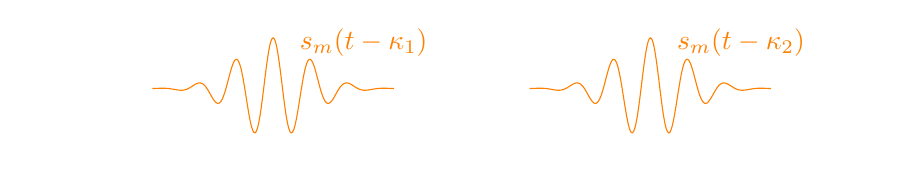
\begin{tikzpicture}[/pgfplots/.cd,width=\columnwidth,height=3cm]
    \begin{axis}[xmin=-0.5,xmax=5,ymin=-1,ymax=1.2,
        xticklabels=\empty,
        yticklabels=\empty,
        axis line style={draw=none},
        tick style={draw=none}]
        %\addplot[no markers,smooth,samples=201,domain=0:2.5, color=white] 
        {exp(-9*(x-1)*(x-1))*cos((x-1)*1440)};

        %\addplot[no markers,smooth,samples=401,domain=0:5, color=white] 
        %{exp(-9*(x-1)*(x-1))*cos((x-1)*1440) + exp(-9*(x-3.5)*(x-3.5))*cos((x-3.5)*1440)};
        %\addplot[no markers,smooth,samples=201,domain=0.2:1.8, color=orange] 
        {exp(-9*(x-1)*(x-1))*cos((x-1)*1440)};
        %\addplot[no markers,smooth,samples=201,domain=2.7:4.3, color=orange] 
        {exp(-9*(x-3.5)*(x-3.5))*cos((x-3.5)*1440)};
        % 

        \addplot[no markers,smooth,samples=2,domain=0:0.2, color=white]
        {exp(-9*(x-1)*(x-1))*cos((x-1)*1440) + exp(-9*(x-3.5)*(x-3.5))*cos((x-3.5)*1440)}; 
        \addplot[no markers,smooth,samples=201,domain=0.2:1.8, color=orange]
        {exp(-9*(x-1)*(x-1))*cos((x-1)*1440) + exp(-9*(x-3.5)*(x-3.5))*cos((x-3.5)*1440)};
        \addplot[no markers,smooth,samples=2,domain=1.8:2.7, color=white]
        {exp(-9*(x-1)*(x-1))*cos((x-1)*1440) + exp(-9*(x-3.5)*(x-3.5))*cos((x-3.5)*1440)};
        \addplot[no markers,smooth,samples=201,domain=2.7:4.3, color=orange]
        {exp(-9*(x-1)*(x-1))*cos((x-1)*1440) + exp(-9*(x-3.5)*(x-3.5))*cos((x-3.5)*1440)};
        \addplot[no markers,smooth,samples=2,domain=4.3:5, color=white]
        {exp(-9*(x-1)*(x-1))*cos((x-1)*1440) + exp(-9*(x-3.5)*(x-3.5))*cos((x-3.5)*1440)};

        {exp(-9*(x-1)*(x-1))*cos((x-1)*1440) + exp(-9*(x-3.5)*(x-3.5))*cos((x-3.5)*1440)};


        \node[text=orange] at (axis cs:1.6,0.9) {$s_m(t-\kappa_1)$};
        \node[text=orange] at (axis cs:4.1,0.9) {$s_m(t-\kappa_2)$};
        \node[color=white] at (axis cs:-0.1,0.4) {$y_m(t)$};

        %\node[color=white] at (axis cs:0.2,-0.3) {$ $};
        %\node[] at (axis cs:0.2,0) {$|$};
        %\node[] at (axis cs:1.8,0) {$|$};
        %\node[color=white] at (axis cs:2.7,-0.3) {$ $};
        %\node[] at (axis cs:2.7,0) {$|$};
        %\node[] at (axis cs:4.3,0) {$|$};

    \end{axis}
\end{tikzpicture}

\begin{tikzpicture}[/pgfplots/.cd,width=\columnwidth,height=3cm]
    \begin{axis}[xmin=-0.5,xmax=5,ymin=-1,ymax=1.2,
        xticklabels=\empty,
        yticklabels=\empty,
        axis line style={draw=none},
        tick style={draw=none}]
        \addplot[no markers,smooth,samples=201,domain=0:2.5, color=white] 
        {exp(-9*(x-1)*(x-1))*cos((x-1)*1440)};

        \addplot[no markers,smooth,samples=201,domain=2.5:5, color=white] 
        {exp(-9*(x-3.5)*(x-3.5))*cos((x-3.5)*1440)};
        \addplot[no markers,smooth,samples=201,domain=0.2:1.8, color=orange] 
        {exp(-9*(x-1)*(x-1))*cos((x-1)*1440)};
        %\addplot[no markers,smooth,samples=201,domain=2.7:4.3, color=orange] 
        {exp(-9*(x-3.5)*(x-3.5))*cos((x-3.5)*1440)};
        % 
        \node[text=orange] at (axis cs:1.6,0.9) {$s_m(t-\kappa_1)$};
        %\node[text=orange] at (axis cs:4.1,0.9) {$s_m(t-\kappa_2)$};
        \node[color=white] at (axis cs:-0.1,0.4) {$y_m(t)$};

        \node[color=white] at (axis cs:0.2,-0.3) {$ $};
        \node[color=white] at (axis cs:0.2,0) {$|$};
        \node[color=white] at (axis cs:2.7,-0.3) {$ $};
        %\node[] at (axis cs:2.7,0) {$|$};
    \end{axis}
\end{tikzpicture}

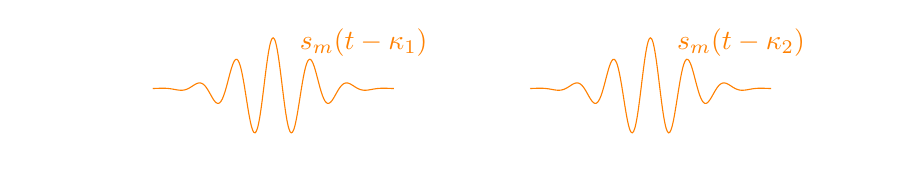
\begin{tikzpicture}[/pgfplots/.cd,width=\columnwidth,height=3cm]
    \begin{axis}[xmin=-0.5,xmax=5,ymin=-1,ymax=1.2,
        xticklabels=\empty,
        yticklabels=\empty,
        axis line style={draw=none},
        tick style={draw=none}]
        \addplot[no markers,smooth,samples=201,domain=0:2.5, color=white] 
        {exp(-9*(x-1)*(x-1))*cos((x-1)*1440)};

        \addplot[no markers,smooth,samples=201,domain=2.5:5, color=white] 
        {exp(-9*(x-3.5)*(x-3.5))*cos((x-3.5)*1440)};
        \addplot[no markers,smooth,samples=201,domain=0.2:1.8, color=orange] 
        {exp(-9*(x-1)*(x-1))*cos((x-1)*1440)};
        \addplot[no markers,smooth,samples=201,domain=2.7:4.3, color=orange] 
        {exp(-9*(x-3.5)*(x-3.5))*cos((x-3.5)*1440)};
        % 
        \node[text=orange] at (axis cs:1.6,0.9) {$s_m(t-\kappa_1)$};
        \node[text=orange] at (axis cs:4.1,0.9) {$s_m(t-\kappa_2)$};
        \node[color=white] at (axis cs:-0.1,0.4) {$y_m(t)$};

        \node[color=white] at (axis cs:0.2,-0.3) {$ $};
        \node[color=white] at (axis cs:0.2,0) {$|$};
        \node[color=white] at (axis cs:2.7,-0.3) {$ $};
        \node[color=white] at (axis cs:2.7,0) {$|$};
    \end{axis}
\end{tikzpicture}
% 
\begin{tikzpicture}[typetag/.style={rectangle, draw, rounded corners,fill=black!70, fill opacity=1, text opacity=1,text width=1.4cm, align=center,minimum width=1cm, minimum height=0.5cm},
    cascaded/.style={double copy shadow={shadow xshift=1ex,shadow yshift=-1ex}},
    sum/.style={draw, circle, fill=black!70, inner sep=5pt},color=white]
        % Nodes
        \node [](input1) {$y_1(t)$};
        \node [right=of input1,sum,xshift=-0.4cm,yshift=-0.795cm] (sum) {$\Sigma$};
        \node [right=of sum,typetag,xshift=-0.4cm] (kurtosis) {Kurtosis};
        
        
        \node (input2)[below=of input1,] {$y_M(t)$};
        
        \node [right=of kurtosis,typetag,xshift=-0.4cm,fill=green!40!black] (event) {Event};

        \node [right=of event,xshift=-0.6cm] (output) {$\hat{z}_{1:M}^n(t)$};
        
        % Arrows
        \draw[->] (input1) -- (sum);
        \draw[->] (sum) -- (kurtosis);
        \draw[->] (kurtosis) -- (event);
        \draw[->] (input2) -- (sum);
        \draw[->] (event) -- (output);

        \path [] (input1) -- node[auto=false]{\vdots} (input2);
        
        \end{tikzpicture}  

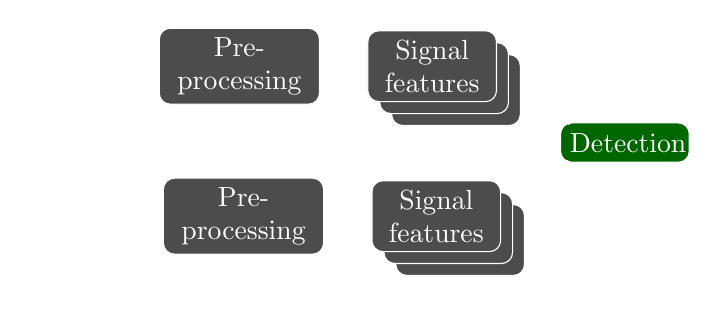
\begin{tikzpicture}[typetag/.style={rectangle, draw, rounded corners,fill=black!70, fill opacity=1, text opacity=1,text width=1.4cm, align=center,minimum width=1cm, minimum height=0.5cm},
    cascaded/.style={double copy shadow={shadow xshift=1ex,shadow yshift=-1ex}},color=white]
        % Nodes
        \node (input1) {$\hat{z}^n_1(t)$};
        \node [right=of input1,typetag,xshift=-0.4cm,text width=1.8cm] (preproc1) {Pre-processing};
        \node [right=of preproc1,typetag,cascaded,xshift=-0.4cm] (signal1) {Signal features};
        
        
        \node (input2)[below=of input1,yshift=-0.3cm] {$\hat{z}^n_M(t)$};
        \node [right=of input2,typetag,xshift=-0.4cm,text width=1.8cm] (preproc2) {Pre-processing};
        \node [right=of preproc2,typetag,cascaded,xshift=-0.4cm] (signal2) {Signal features};
        
        \node [right=of signal1,typetag,yshift=-0.97cm,xshift=-0.2cm,fill=green!40!black] (detection) {Detection};
        \node [below=of signal2,yshift=0.8cm] (dummy) {};
        
        % Arrows
        \draw[->] (input1) -- (preproc1);
        \draw[->] (preproc1) -- (signal1);
        \draw[->] (signal1) -- (detection);
        \draw[->] (input2) -- (preproc2);
        \draw[->] (preproc2) -- (signal2);
        \draw[->] (signal2) -- (detection);
        \path (input1) -- node[auto=false]{\vdots} (input2);
        
        \node [right=of preproc1,typetag,cascaded,xshift=-0.4cm] (signal1) {Signal features};
        
        \end{tikzpicture}
% \begin{tikzpicture}[thick, scale=0.7]
%     \node at (2,0) (LowerRight) {};
%     \node at (-2,0) (LowerLeft) {};
%     \node at (0,3.464) (Top) {};
%     \node at (0,1.1547) (Center) {};
%     \draw[orange, dashed,ultra thick] (LowerRight) -- (LowerLeft);
%     \draw[orange, dashed,ultra thick] (LowerRight) -- (Top);
%     \draw[orange, dashed,ultra  thick] (LowerLeft) -- (Top);
%     \filldraw[black] (LowerLeft) circle (10pt) {};
%     \node[white] at (LowerLeft) {$1$};
%     \filldraw[black] (LowerRight) circle (10pt)  {};
%     \node[white] at (LowerRight) {$2$};
%     \filldraw[black] (Top) circle (10pt)  {};
%     \node[white] at (Top) {$3$};

%     \draw[black,ultra thick, <->,yshift=0.65*0.5cm,,xshift=-0.65*0.866cm] (-2,0) -- (0,3.464) node[midway,above,black,rotate=60] {$4$\,m};

%     \filldraw[gray] (Center) circle (5pt) {};
%     \draw[gray,ultra thick] (Center) -- (2,1.1547);
%     \draw[gray,dotted,ultra thick] (Center) -- (2,1.1547+2);
%     \draw[->, gray,ultra thick] (1.5,1.1547) arc
%         [
%             start angle=0,
%             end angle= 45,
%             x radius= 1.5cm,
%             y radius =1.5cm
%         ] node[midway,right,gray] {$\phi(t)$};
% \end{tikzpicture}

\end{document}